

\newpage
\section{Berita lingkungan tahun 2017}
Awal tahun ditandai dengan perayaan Natal lingkungan sekaligus sebagai ungkapan syukur umat St. Theresia atas tahun yang baru.

\subsection*{Prapaskah}
Prapaskah lingkungan diadakan setiap Kamis pada masa Prapaskah. Pada acara tersebut dipandu oleh tim dan diadakan \textit{sharing}. Umat St. Theresia cukup antusias dalam mengikuti acara ini. Pada saat acara dilaksanakan banyak umat yang dengan semangat men-\textit{sharing}-kan pengalaman imannya. 

\subsection*{Paskah Lingkungan}
Paskah lingkungan St. Theresia diselenggarakan pada tanggal 23 April 2017 hari Minggu jam 19.00. Acara dikelola oleh OMK St. Theresia. Acara tersebut mengangkat tema \textit{\textbf{berbagi antar sesama}} dengan diawali pembagian kelompok. Setiap kelompok ditugasi membuat hiasan roti sebaik-baiknya. Tanpa pemberitahuan sebelumnya, hasil roti hiasan kemudian diminta untuk diberikan kepada orang lain dari kelompok lain, yang bermakna bahwa memberi kepada orang lain mestinya barang atau karya yang terbaik. 

Acara juga diisi dengan kuis berhadiah antara lain berupa tebak lagu dan juga tebak gambar.

\subsection*{Kirab salib AYD}

\begin{floatingfigure}[r]{1.7cm}
	\begin{center}
		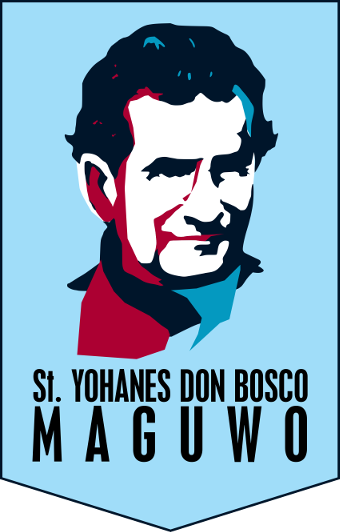
\includegraphics[scale=0.15]{don-bosco-025.png}
	\end{center}
\end{floatingfigure}


Sehubungan dengan kirab salib AYD,setiap wilayah di Paroki Marganingsih Kalasan diwajibkan membuat vandel atau panji-panji dengan ukuran dan format yang sudah ditentukan. Lingkungan St. Theresia masuk dalam wilayah St. Yohanes Don Bosco. Desain vandel dilakukan oleh Ade, warga St. Theresia dan hasil akhirnya berupa vandel dengan bahan kain satin berbordir. 

\subsection*{Rosario dan BKL}
%termasuk Novena Roh Kudus
Bulan Mei adalah Bulan Maria. Tidak ketinggalan umat lingkungan St. Theresia turut serta menyambut Bulan Maria dengan mengadakan Doa Rosario setiap hari. Dalam kesempatan doa ini, juga dilaksanakan kegiatan Bulan Katekese Liturgi (BKL). Setiap tahun Keuskupan Agung Semarang (KAS) menyediakan panduan untuk kegiatan ini. Panduan disusun untuk disampaikan setiap hari di bulan Mei.

Doa Rosario diadakan bergantian di rumah umat. Setiap keluarga umumnya mendapat 1 kali kesempatan menjadi tempat doa rosario. Karena jumlah keluarga kurang dari 31 maka selain di rumah-rumah keluarga, doa rosario bertempat di Joglo Lawas. 

BKL dipandu oleh tim yang sudah mempersiapkan diri. Biasanya dalam kegiatan ini terjadi dialog antara umat dengan pemandu maupun umat dengan umat. Beberapa kesempatan umat menyampaikan pertanyaan dan pemandu akan menjawab, jika tahu jawabannya. Namun demikian tidak menutup kemungkinan yang memberi jawaban adalah umat lain. 

\subsection*{Ziarah ke Sendang Sriningsih}
Ziarah dilaksanakan pada tanggal 28 Mei 2017 dengan panitia diketuai oleh Bapak Heru Pratomo. Perjalanan dilakukan dengan menggunakan 10 mobil milik umat St. Theresia dengan peserta sejumlah 49 orang. Berangkat kira-kira jam 10 pagi dan kurang lebih 1 jam kemudian sudah sampai tujuan.

Sendang Sriningsih berada di Jali dan masuk dalam paroki Wedi Klaten. Sendang ini sudah cukup lama dan banyak pengunjung terutama pada malam Jumat Kliwon menurut hari pasaran Jawa.


\subsection*{Ulang tahun GBM}
Misa ulang tahun GBM diselenggarakan pada tanggal 10 Juni 2017, hari Sabtu jam 17.00. Kebetulan pada waktu itu lingkungan St. Theresia mendapat tugas koor. Karena bertepatan dengan hari ulang tahun GBM maka tugas itu didukung juga oleh kelompok D'Amor.

Setelah misa dilanjutkan dengan pesta rakyat yang menyajikan makanan spesial \textit{bakmi godhog} alias mi rebus. Setiap lingkungan wajib menyediakan menu itu dan sebagai juru masak untuk lingkungan St. Theresia dilaksanakan oleh Ibu A. Sri Supriyati, yang memang sudah biasa dan senang memasak.

\subsection*{Komuni Pertama}
Komuni pertama untuk Lily (Regina Kalyca Damastus), Abi (Ignatius Abimanamanasa), dan Sasya (Anatasya Bunga Rosari) tanggal 18 Juni 2017. Lily menerima komuni pertama di Gereja Kristus Raja Baciro sedang Sasha di Gereja Bunda Maria Maguwo.

Lily adalah anak pertama dari pasangan V. Dalyono dan V. Indah Kartikasari, sedangkan Sasha adalah anak kedua dari pasangan C. Triyono dan Y. Jatiningsih. Sementara itu Abi merupakan salah satu keluarga dari Bapak Anton Supriyana.

Tanggal 22 Juni 2017 bertepatan dengan doa lingkungan diserahkan kenang-kenangan kepada ketiga anak penerima komuni pertama. Kenang-kenangan yang berupa buku-buku rohani diserahkan oleh Ketua Lingkungan.

\subsection*{BKSN 2017}
BKSN tahun 2017 diselenggarakan pada bulan September seperti tahun-tahun sebelumnya. Setiap Kamis jam 19.00 pada bulan itu BKSN diadakan di rumah keluarga Paulus Suroyo. Tahun ini BKSN bertema Dalam konteks meneliti dan menanggapi tantangan yang dihadapi oleh dunia modern yang akhirnya juga ikut melanda Gereja, Bulan Kitab Suci Nasional tahun 2017 mengambil tema, “Kabar Gembira Di Tengah Gaya Hidup Modern.” 

Tema ini dijabarkan dalam empat sub tema. Pertama, arus zaman teknologi dan nilai-nilai injili dalam kisah menara Babel (Kej. 11:1-9). Kedua, arus zaman materialisme dan nilai-nilai injili dalam perumpamaan orang kaya yang bodoh (Luk. 12:13-21). Ketiga, arus zaman individualisme dan nilai-nilai injili dalam kisah cara hidup jemaat perdana (Kis. 2:41-47). Keempat, arus zaman hedonisme dan nilai-nilai injili dalam nasihat Yakobus tentang hikmat dan hawa nafsu (Yak. 3:14-4:3). Melalui keempat sub tema ini diharapkan umat kristiani tidak terseret dan terhanyut oleh arus zaman modern dengan terus berpegang pada nilai-nilai injili.

Pelaksanaan BKSN dipandu oleh tim yang sudah ditunjuk oleh ketua lingkungan. BKSN berlangsung dalam format diskusi atas kisah pendukung topik dan renungan serta doa umat. Diskusi berlangsung dalam bentuk \textit{sharing} pengalaman maupun \textit{sharing} pengetahuan.

\subsection*{Nonton bareng film 'Yesus menurut Injil Yohanes}

Film 'Yesus menurut Injil Yohanes' yang didapat dari Youtube atas informasi dari Bu Nanik, diputar pada hari Rabu 27 September 2017 di Joglo Lawas. Selain warga St. Theresia diundang dan hadir pula warga dari lingkungan St. Petrus dan St. Monica. Walaupun durasi film sepanjang 3 jam lebih namun sebagian besar penonton bertahan sampai habis. Bahkan setelah itu masih dilanjutkan dengan ngobrol bersama. 

Film ini mengisahkan Yesus seperti yang tertulis dalam Injil Yohanes. Dengan melihat film ini para penonton bisa lebih menghayati Injil Yohanes dan Sabda Tuhan yang ada dalam Injil Yohanes. 

\subsection*{Peringatan 1 tahun meninggalnya Ibu Theresia Suci Wahyuningsih}
Pada akhir bulan September atau tepatnya tanggal 30, keluarga Anton Supriyana mengundang warga St. Theresia untuk menghadiri misa peringatan 1 tahun Ibu Theresia Suci Wahyuningsih dipanggil Tuhan. Selain warga lingkungan St. Theresia juga hadir warga lingkungan St. Monica dan St. Petrus, beserta keluarga dan sahabat keluarga Anton Supriyana. Misa dipimpin oleh Romo Bambang yang seperti biasa membawa kesegaran dalam homilinya.

Dalam kesempatan tersebut untuk pertama kalinya Maria Rosa Firanti (Fira) bertugas mengiringinya dengan \textit{keyboard} untuk semua lagu dalam misa. Pada saat itu Fira didampingi oleh Pak Andre sehingga lebih percaya diri.


\subsection*{Lomba BKSN di Paroki Marganingsih}
Dalam rangka BKSN tahun 2017, OMK paroki mengadakan pancalomba tentang liturgi dan kitab suci. Mata lomba meliputi: lektor, pemazmur, tata liturgi, cerdas cermat alkitab, dan visualisasi kitab suci. Lomba diadakan pada hari Minggu 8 Oktober 2017.

Lingkungan St. Theresia mengirim 3 wakilnya sekaligus mewakili GBM.  Mereka adalah Anastasya Bunga Rosari (Sasya), 
Aditya Riani Widwianingrum (Riani), dan 
Petrus Krisologus Hargyan Revano (Hagi).
Sasya adalah anak kedua dari keluarga C. Triyono, sedangkan Riani anak kedua juga namun dari keluarga P. Suroyo. Hagi adalah warga baru dan merupakan anak ketiga dari keluarga Y. Saptanto SB.

Dalam kesempatan tersebut Sasya dan Riani ikut dalam mata lomba lektor sedangkan Hagi ikut dalam mata lomba pemazmur. Hagi berada dalam keluarga yang senang menyanyi dan rata-rata memiliki suara bagus. Kakaknya ikur juga dalam paduan suara kampus. Sasya beberapa kali ditugasi sebagai pembaca Alkitab dalam pertemuan lingkungan. Bersama dengan teman-teman lainnya beberapa kali pula memimpin doa rosario lingkungan.

Riani sudah terbiasa ditugasi sebagai pembaca Alkitab dalam pertemuan-pertemuan lingkungan. Pernah juga tugas sebagai lektor di perayaan ekaristi di Gereja Bunda Maria Maguwo. Dalam lomba ini Riani mendapat juara ketiga. 

\subsection*{Ziarah ke Sendang Ratu Kenya Wonogiri}
Sendang Ratu Kenya Wonogiri merupakan salah satu tempat ziarah yang banyak didatangi pada bulan Maria dan bulan Rosario. Tahun 2017 ini umat St. Theresia berkesempatan ziarah ke tempat tersebut bersama-sama dengan umat dari lingkungan St. Monika dan St. Petrus pada tanggal 15 Oktober 2017. Berangkat dari GBM pukul 6.30 menggunakan bis langsung menuju Sendang Ratu Kenya. Kira-kira jam 9.30 sudah sampai di tujuan, istirahat sejenak kemudian berjalan kaki menuju awal perhentian jalan salib. 

Tidak begitu padat peziarah saat itu, tetapi karena antar perhentian hanya berjarak pendek maka sesekali terjadi penumpukan 2 atau 3 kelompok ziarah di satu perhentian. Akhir jalan salib dilanjutkan dengan doa pribadi masing-masing di depan gua Maria ataupun di depan kapel. 
Setelah sempat cuci muka, cuci kaki, dan pasang lilin, dan beristirahat sejenak, perjalanan dilanjutkan ke pantai Baron. 

Seperti biasa pantai Baron selalu penuh pengunjung. Banyak warung-warung makanan dan cindera mata. Beberapa umat sempat liaht-lihat pemandangan di pantai yang sudah dipadati pengunjung. Beberapa umat menyempatkan diri makan siang, minum kopi, atau sekedar beli oleh-oleh.

Perjalanan dari Baron kembali pulang cukup lancar. Namun sedikit tersendat saat menjelang Patuk. Ternyata di daerah itu banyak bunga amarilis sedang mekar sehingga memancing pengguna jalan untuk memperlambat kendaraannya agar bisa menikmati keindahan bunga amarilis yang mekar berbarengan.

\subsection*{Pesta Nama dan Penutupan Bulan  Rosario}
Di akhir bulan Oktober 2017 tepatnya tanggal 31, warga lingkungan St. Theresia mengadakan misa syukur atas penyelenggaran Doa Rosaria bersama selama 1 bulan dengan lancar. Misa syukur juga dimaksudkan sebagai pesta nama lingkungan yang mestinya jatuh pada tanggal 1 Oktober. Sesuai kebiasan di lingkungan, pesta nama disatukan dengan penutupan bulan rosario. 

Misa dipimpin oleh Rm Ambrosius Wagiman Wignyosumantoro Pr., Romo Paroki Marganingsih Kalasan, dimulai pukul 18.00. Dalam homilinya Romo menyampaikan bahwa kesederhanaan, kesetiaan pada orang kecil, dan kesetiaan kepada Yesus, yang ditunjukkan oleh Santa Theresia patut diteladani oleh warga lingkungan.

Seusai misa dilanjutkan dengan acara potong tumpeng oleh Romo dan diserahkan kepada ketua lingkungan Bapak Anton Supriyana. Romo juga sempat menyerahkan bingkisan kenang-kenangan kepada peserta lomba Bulan Kitab Suci di Paroki yaitu Riani, Hagi, dan Sasya. Pada kesempatan tersebut juga diserahkan bingkisan kepada Fira dan Abi atas keberaniannya. Fira telah berani mengiringi koor dan Abi telah berani menjadi putra altar.

Sambil makan nasi kuning dan nasi tumpeng acara masih berlanjut dengan pembagian hadiah pemenang lomba untuk memeriahkan pesta nama lingkungan. Juara lomba ping pong tunggal diraih oleh Pak Yanto, Pak Gelung, dan Pak Andre. Juara lomba ping pong ganda diraih oleh Bu Mia/Bu Kris, Pak Anton/Pak Neo, dan Pak Darmadi/Bu Andre. Di lomba catur juara diraih oleh Pak Neo, Phito, dan Pak Sandy.

Pada acara tersebut tampil juga biola tunggal yang dimainkan oleh Lintang. Ada juga pembagian \textit{door prize} untuk anak-anak dan juga orang tua.

\subsection*{Adven}
Ibadat tahun 2017 seperti pada tahun-tahun sebelumnya diisi dengan \textit{sharing} tentang suatu tema.
Tema tahun 2017 adalah \textit{DALAM TERANG IMAN, MENGHIDUPI NILAI-NILAI PANCASILA}. 
Berhubung hari Minggu terakhir Adven jatuh pada tanggal 24 Desember maka ibadat Adven dimulai sebelum hari Minggu Adven pertama.

Pertemuan I
dengan topik \textit{\textbf{Menjunjung Nilai
Ketuhanan Yang Maha Esa
Dalam Menggereja dan
Berbangsa}}
dilaksanakan pada tanggal 30 November 2017 bertempat di rumah Bapak FX Sularto. Ibadat dan \textit{sharing} dipimpin oleh Bapak Neo Suradi. Dalam pertemuan ini ditegaskan bahwa sebagai Bangsa Indonesia, nilai Ketuhanan
yang Maha Esa, juga berarti sebuah sikap hormat dan
memberi jaminan kebebasan kepada setiap penduduk atau
warga bangsa untuk memeluk agama sesuai dengan
keyakinannya dan beribadah menurut kepercayaannya masing-masing.

Pertemuan II dengan topik \textit{\textbf{Menjunjung Nilai Kemanusiaan
		Dalam Tata Hidup Bersama
}} dilaksanakan di Joglo Lawas berhubung keluarga FX Sularto sedang prihatin karena kerabat dekatnya sakit pada tanggal 7 Desember 2017.

Dalam pertemuan ini dibahas tentang Sila kedua dan kelima dari Pancasila. Dalam Ajaran Sosial Gereja, nilai kemanusiaan dan
keadilan sangat mendasar, karena Gereja Katolik
menjunjung tinggi setiap martabat manusia. Ajaran Sosial Gereja mengatakan bahwa setiap pribadi manusia itu
luhur, karena setiap darinya diciptakan Allah. Siapapun
manusia telah dilahirkan memiliki keluhuran yang tak
tergantikan. Allah telah memberikan karunia keluhuran
bagi setiap pribadi sebagai anugerah yang sudah diberikan
sebelum manusia dilahirkan di dunia ini. Maka, nilai-nilai
Pancasila menyangkut kemanusiaan dan keadilan dalam
nafas Gereja Katolik juga mendapatkan arti dan
pemaknaan yang sama. Keluhuran martabat manusia
itulah dasar dari hak asasi manusia. Martabat manusia
selalu melekat dalam hak paling asasi manusia. Hal itu
harus dibela tidak hanya secara individual tetapi juga
sebagai keseluruhan di dalam hidup bermasyarakat dan
berbangsa.


Pertemuan III diadakan pada tanggal 14 Desember 2017 di rumah Bapak FX Sularto dipimpin oleh Ibu Th Nanik Ismarjiyati dengan topik \textit{\textbf{Menjunjung Nilai Persatuan dan
		Musyawarah Dalam Hidup
		Bermasyarakat dan Bernegara
}}.
	
Gereja Katolik melalui Ajaran Sosial Gereja juga
mengangkat nilai-nilai yang sama mengenai rasa cinta
bangsa, persatuan, gotong royong dan musyawarah.
Dalam Ajaran Sosial Gereja, secara khusus dari Centesimus Annus, artikel 46, dikatakan bahwa Gereja
menghargai sistem demokrasi, sehingga Gereja Katolik
juga menjunjung hak tiap orang untuk ambil-bagian dalam
hidup masyarakat dan bernegara, khususnya dalam peran
serta politik. Begitu juga dalam Gaudium Et Spes artikel
76, Gereja juga mengajak umat Katolik dengan setia
menjunjungtanggungjawab hidup bernegara dan
mengutamakan musyawarah harus dijunjung tinggi.

Pertemuan IV dipimpin oleh Bapak Andre Muda bertempat di rumah Bapak FX Sularto pada tanggal 21 Desember 2017. Ini pertemuan terakhir Adven tahun 2017.	
	
\subsection*{Jagong Bayi Yesus}
Gereja Bunda Maria memulai tradisi baru dengan mengadakan acara \textit{Jagong Bayo Yesus}. Acara ini dilaksanakan mulai tanggal 25 Desember 2017 sampai dengan 5 Januari 2018. Setiap lingkungan di GBM mendapat jatah 1 hari. Lingkungan Theresia mendapat jatah tanggal 29 Desember 2017. Umat lingkungan berkehendak bahwa acara jagong bayi ini juga sekaligus sebagai perayaan Natal lingkungan. Acara dimulai jam 19.00 dengan melakukan doa bersama di depan gua natal. Setelah itu dilanjutkan dengan ramah-tamah di gazebo sampai dengan pukul 21.00.	
